\documentclass[bibliography=totoc, 12pt, a4paper, twoside]{scrartcl}

\usepackage{scrlayer-scrpage}
\setkomafont{pageheadfoot}{\sffamily\footnotesize}
\setkomafont{pagination}{}
\ofoot*{Seite~\pagemark}

\usepackage[margin=2.5cm]{geometry}      % Sets page margins to be of 2.5cm
\usepackage[ngerman]{babel}              % Sets local preferences for german region
\usepackage[style=iso-numeric]{biblatex} % package for citation management
\usepackage{svg}                         % included for svg inclusion of HSE-Logo
\usepackage{graphicx}
\graphicspath{{./Grafiken/}}
\usepackage{float}
\usepackage[font=footnotesize]{caption}
\usepackage{hyperref}                    % Useful for Links
\usepackage{siunitx}
\usepackage{subcaption}

\setlength{\parindent}{0pt}              % Sets the value, with which each paragraph is indented; deactivated
\setlength{\parskip}{1em}                % Sets the value of space in between two paragraphs
\linespread{1.25}

\addbibresource{bibliography.bib}

\titlehead{Hochschule Esslingen\\Flandernstraße 101\\73732 Esslingen a. N.}
\subject{Ausarbeitung --- Sensoren und Aktoren}
\title{BLDC-Motoren}
\subtitle{Technische Varianten und Anwendungen}
\author{Emil Slomka\thanks{\href{mailto:emslit01@hs-esslingen.de}{\nolinkurl{emslit01@hs-esslingen.de}}} \and Tim Hilt\thanks{\href{mailto:tihigl00@hs-esslingen.de}{\nolinkurl{tihigl00@hs-esslingen.de} }}}
\date{\today}
\publishers{Betreut durch Herrn Professor Reinhard Keller}

%%% Local Variables:
%%% mode: latex
%%% TeX-master: "BLDC"
%%% End:


\begin{document}

\maketitle
\thispagestyle{empty}
\cleardoublepage
\pagenumbering{arabic}
\tableofcontents
\clearpage
\listoffigures
\clearpage

\section{Einleitung}

%%% Local Variables:
%%% mode: latex
%%% TeX-master: "BLDC"
%%% End:

\section{Namensgebung und Abgrenzung zum bürstenbehafteten Gleichstrommotor}

Die englische Bezeichnung \glqq{}BLDC\grqq{} (Brushless-Direct-Current-Motor) bedeutet im Deutschen \glqq{}bürstenloser Gleichstrommotor\grqq{}. Um zu verstehen, weshalb der von uns beschriebene Motortyp diesen Namen trägt wollen wir zunächst auf seinen Vorläufer --- den bürstenbehafteten Gleichstrommotor eingehen und die beiden Motorentypen im Verlauf der Arbeit weiter voneinander abgrenzen.

Bürstenbehaftete Gleichstrommotoren werden auch als \emph{mechanisch kommutierte Gleichstrommotoren} bezeichnet. Diese \glqq{}werden als permanenterregte Nebenschlussmotoren ausgelegt. Sie zeichnen sich durch einen linearen Strom–Drehmoment Verlauf aus, der von der Winkellage des Rotors nahezu unabhängig ist\grqq{} \parencite[S. 51]{Probst2011}. Hier werden mehrere Eigenschaften dieses Motortyps deutlich. Der bürstenbehaftete Gleichstrommotor ist mechanisch kommutiert. Das bedeutet, dass durch Kontaktierung zweier leitender Materialien Strom durch die Motorwicklungen fließen und der Motor sich so drehen kann.

\begin{figure}[H]
  \centering
  \includegraphics[width=8cm]{./Grafiken/AufbauBürstenbehafteterGleichstrommotor}
  \caption[Aufbau bürstenbehafteter Gleichstrommotor]{Prinzipaufbau des bürstenbehafteten Gleichstrommotors (Quelle: \parencite[S. 51]{Probst2011})}
  \label{fig:AufbauBürstenbehaftet}
\end{figure}

Dieser Aufbau hat einige Vorteile. So ist zum Beispiel die Steuerung der Drehzahl und -richtung des Motors durch Variation der Ankerspannung sehr einfach zu realisieren. Auch regelungstechnisch bietet dieser Motortyp aufgrund des linearen Strom-Drehmoment-Verhaltens große Vorteile. Die Herstellung des Motors ist aufgrund insbesondere dieser beiden Eigenschaften sehr kostengünstig umzusetzen. \glqq{}Große Drehzahlstellbereiche bis zu 1:10000 und eine hohe Gleichlaufgüte\grqq{} \parencite[S. 51]{Probst2011} sind weitere positive Eigenschaften, die dem bürstenbehafteten Gleichstrommotor eine klare Daseinsberechtigung bescheinigen.

Der in Abbildung \ref{fig:AufbauBürstenbehaftet} dargestellte Aufbau des bürstenbehafteten Gleichstrommotors zeigt im unteren und oberen Bereich jeweils eine Kohlebürste. Diese aus Graphit bestehenden Bauteile werden mithilfe einer Feder durchgehend auf den Kommutator gedrückt. Beginnt Strom zu fließen, so beginnt sich der Motor zu drehen. Da die Bürsten nach wie vor auf den Kommutator drücken entsteht Reibung und infolgedessen eine mechanische Abnutzung.

\glqq{}Im  Vergleich  zu  anderen  Motorkonzepten  ergeben  sich  die  wesentlichen negativen Eigenschaften des bürstenbehafteten Motors aus seinem prinzipiellen Aufbau\grqq{} \parencite[S. 52]{Probst2011}. Diese negativen Eigenschaften beinhalten zum einen die mechanische Abnutzung und die daraus resultierende Notwendigkeit verschlissene Bürsten zu ersetzen, als auch Reibungsverluste und Probleme mit der Abführung von Abwärme, die durch die mechanische Kommutierung entstehen. Hinzu kommen Nachteile durch unvermeidbare Übergangswiderstände von den Kohlebürsten zum Kommutator. Dadurch wird der maximal mögliche Ankerstrom im Stillstand (Durchbrennen), als auch bei hohen Drehzahlen (Bürstenfeuer) begrenzt \parencite[vgl.][S. 52]{Probst2011}. Diese Effekte können insbesondere im explosionsgefährdeten Arbeitsumfeld lebensbedrohlich werden.

Trotz dieser Nachteile wurde der bürstenbehaftete Gleichstrommotor nicht vollständig durch andere Motorenkonzepte verdrängt, denn insbesondere bei Applikationen mit kostenkritischen Anforderungen und wenig mechanischer Belastung können seine Vorteile hervorragend genutzt werden.

Im Folgenden wird nun die Funktionsweise unterschiedlicher \emph{bürstenloser} Gleichstrommotorentypen erklärt

%%% Local Variables:
%%% mode: latex
%%% TeX-master: "BLDC"
%%% End:

\section{Technische Varianten}

Die Anforderungen an bürstenlose Permanentmagnetantriebe sind sehr vielfältig. Aus diesem Grund werden die verschiedenen Antriebsaufgaben durch unterschiedliche Motorkonstruktionen gelöst. Bei der Auswahl einer geeigneten Motorbauform stehen verschiedenen Kriterien, wie der zur Verfügung stehende Platz, Länge beziehungsweise Durchmesser des MotorS.  Hierzu werden die Anforderungen auf unterschiedliche Betriebsarten festgelegt. Es ist wichtig ob der Motor eine konstante Drehzahl haben soll. Welcher Drehzahlstellbereich, wie sich die Motordynamik verhalten oder ob er rund laufen soll. Eine wichtige Rolle spielt auch die mechanische Stabilität und Schwingungsneigung. Zudem steht auch die Integrationsfähigkeit in eine vorhandene Konstruktion im Bereich der Auswahlkriterien \parencite[S. 74]{Stölting2011}.

In diesem Kapitel werden wichtige Eigenschaften von vier verschiedenen BLDC-Motorbauformen näher bertachtet. Es wird einzeln beschrieben wie die Motoren mit Internal/External-Rotor, Disk-Rotor und der nutenlose Motor funktionieren.

\subsection{Innenläuferausfürung}
Die Innenläuferausführung des bürstenlosen Permanentmagnetmotors entspricht den Vorstellungen einer klassischen Motorausführung, wie man sie in überwiegender Anzahl auch bei den Gleichstromkommutatormotoren und Asynchronmotoren vorfindet.

Das Längen/Durchmesserverhältnis der Läuferausführungen variiert in der Praxis sehr stark von schlanken bis hin zu nahezu scheibenförmigen Rotorkonstruktionen. Im Allgemeinen erlaubt jedoch eine schlanke Konstruktion eine bessere Ausnutzung des magnetischen Kreises, da die magnetischen Streuflüsse an den Stirnseiten sowie die Wickelkopfverluste weniger stark ins Gewicht fallen. Dank Permanentmagneten lassen sich mit der Innenläuferbauform hohe Drehmoment-Trägheitsmoment-Verhältnisse und damit sehr gute dynamische Eigenschaften erzielen.

\begin{figure}[h]
    \centering
    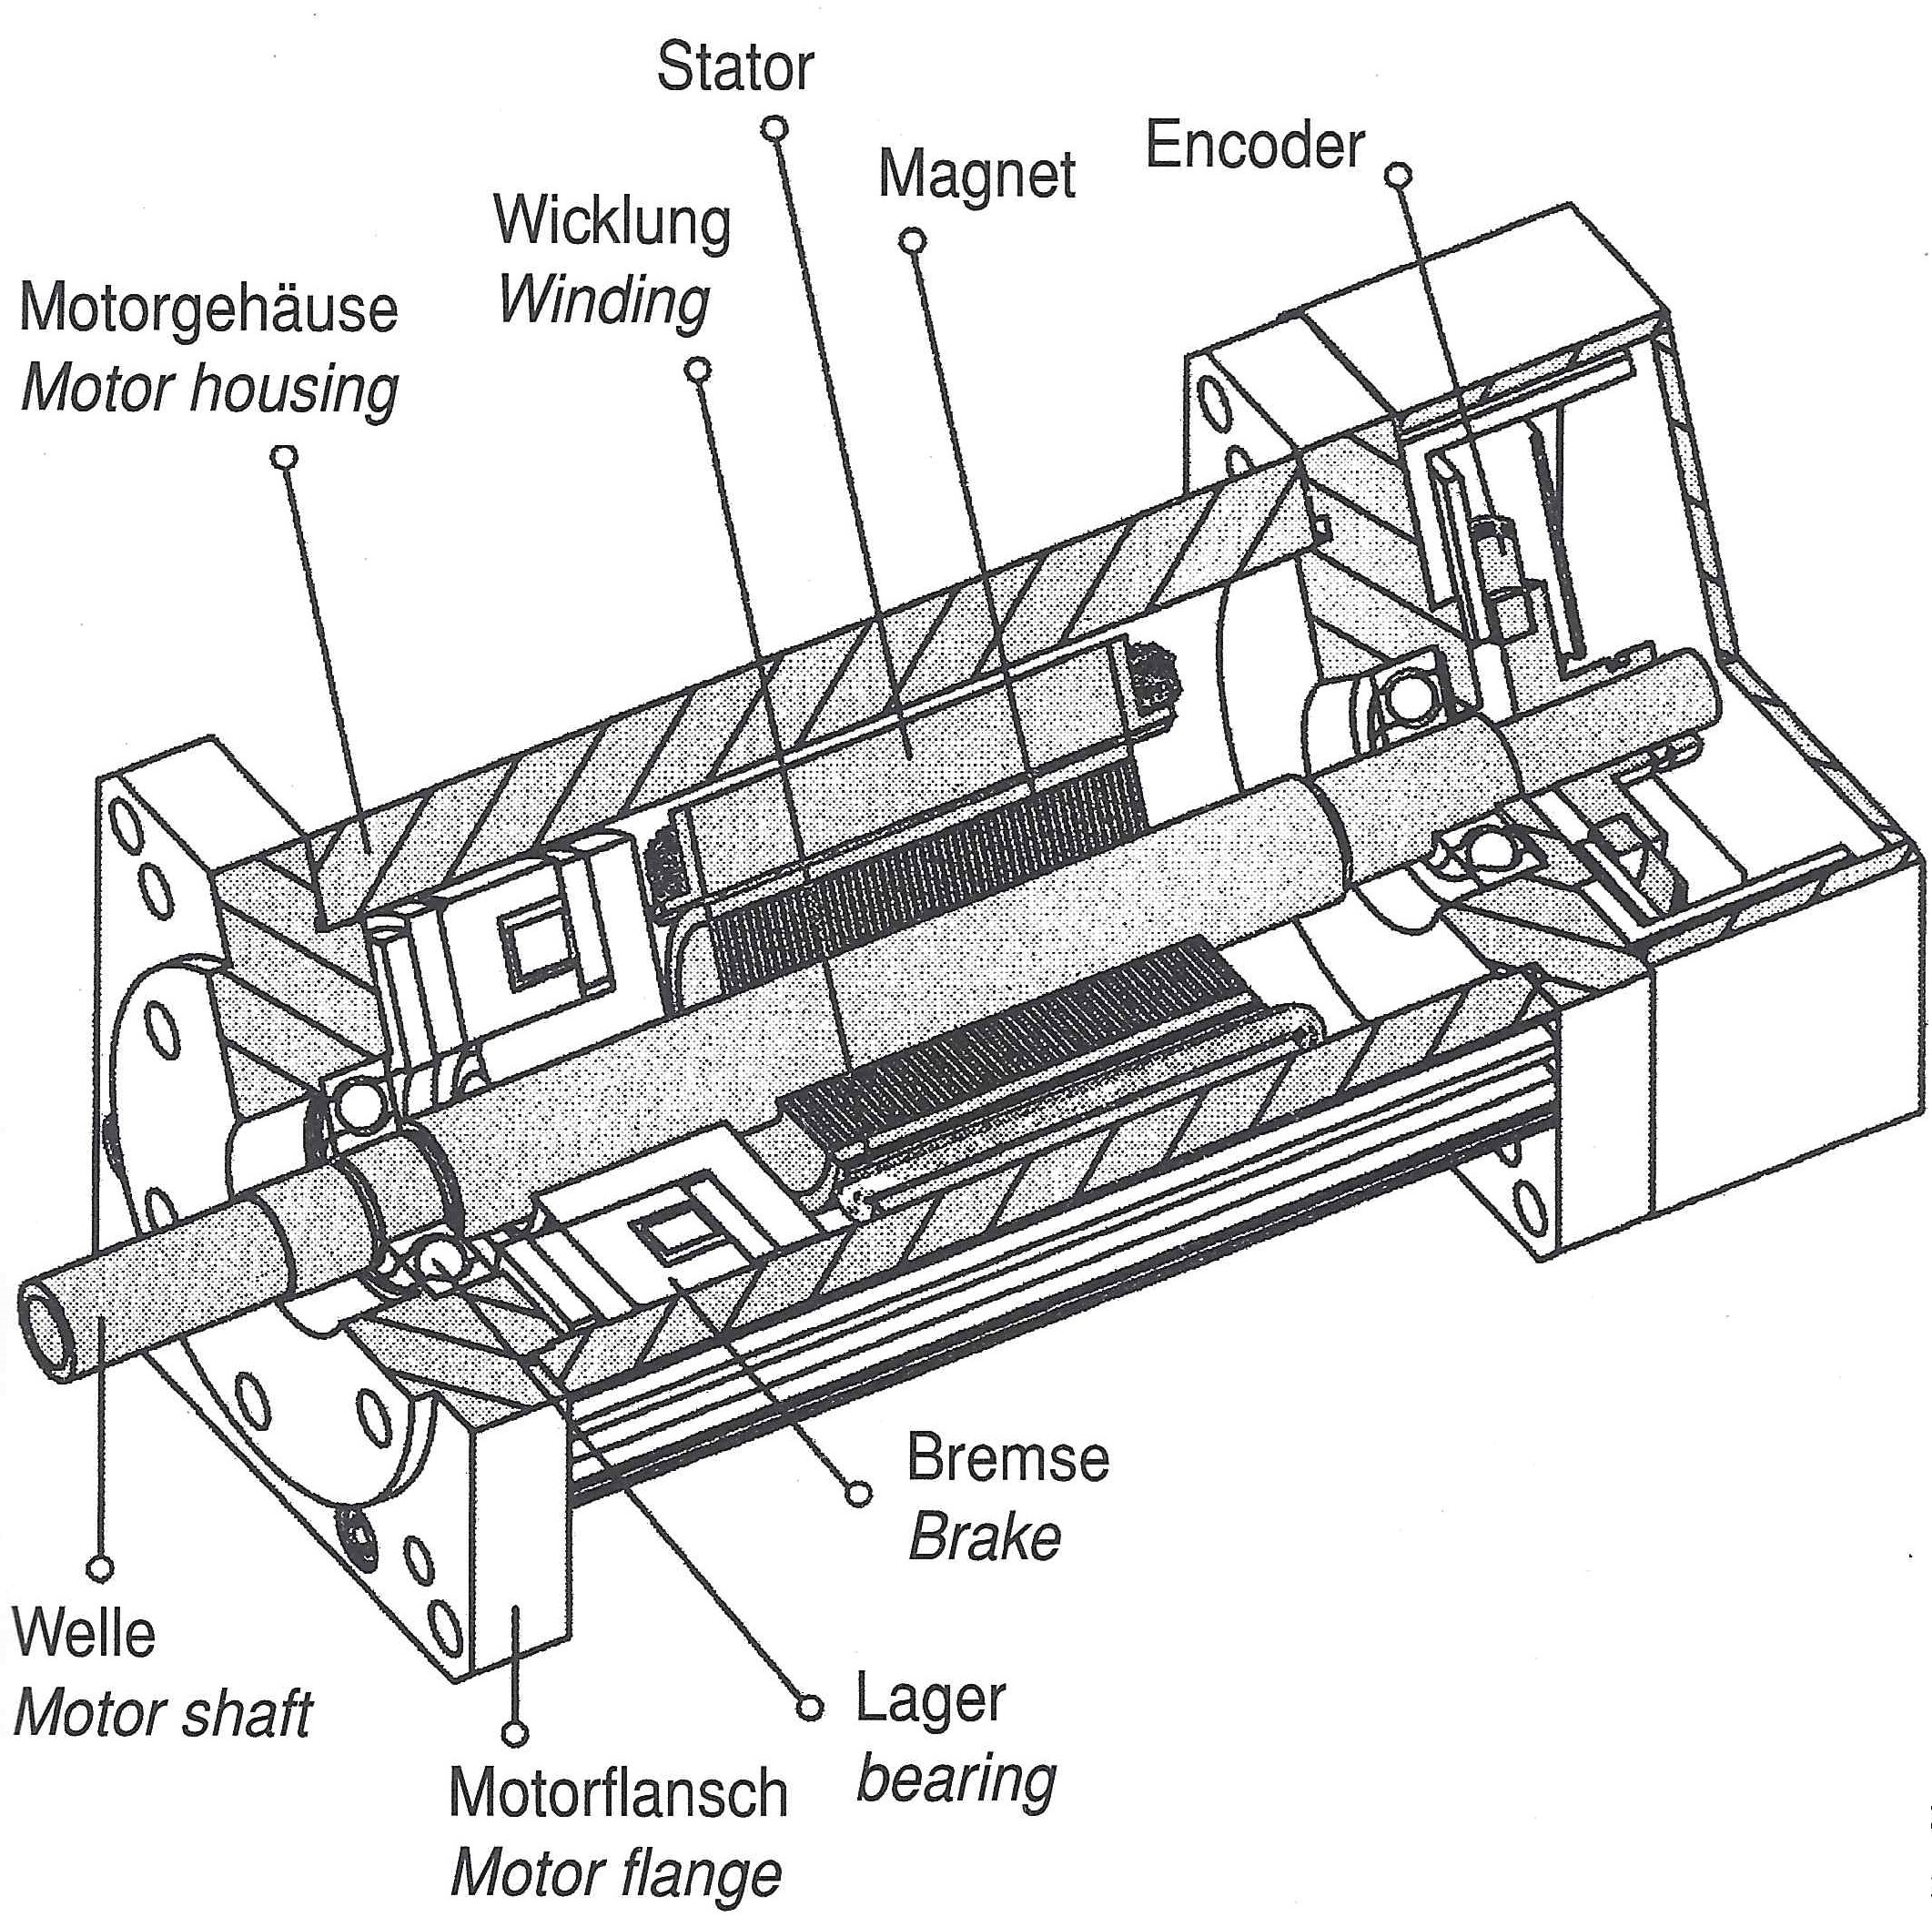
\includegraphics[width=8cm]{./Grafiken/3_1}
    \caption[Schnittbild eines BLDC-Motors in Innenläuferausführung]{Schnittbild eines BLDC-Motors in Innenläuferausführung (Quelle: \parencite[S. 75]{Stölting2011})}
    \label{fig:3_1}
  \end{figure}

Der prinzipielle Aufbau eines permanentmagnetbestückten Innenläufermotors ist in der Abbildung \ref{fig:3_1} zu sehen. Werden die spröden und im magnetisierten Zustand unter hoher, innerer Spannung stehenden Permanentmagnete nicht mechanisch geschützt, so werden sie unter Umständen durch große Fliehkräfte zerstört. Um diesen Effekt zu umgehen werden werden die Segmente beziehungsweise Ringe mithilfe von epoxydharzgetränkten Glas- oder Kohlefasern bandagiert. Zum Teil werden hierzu auch dünngezogene magnetische Nichtstahl- oder Aluminiumhülsen verwendet.

Für den magnetischen Rückschluss im Rotor ist es bei kleinen Statornutöffnungen und großen Magnethöhen meist nicht erforderlich, den Magnetträger zu blechen. Dennoch ist dies in vielen Fällen die kostengünstigste Lösung, zumal das Rotorblech aus dem Kern des Statorblechschnittes im gleichen Arbeitsgang gestanzt werden kann. Bei besonders engen räumlichen Verhältnissen wird die Welle zur magnetischen Leitung des Flusses mit verwendet. In diesen Fällen ist jedoch zu beachten, dass im Gegensatz zu den weichmagnetischen Blechen in der Regel keine eng tolerierten magnetischen Daten des Wellenwerkstoffes vorliegen. Wellen sind grundsätzlich für die Führung des magnetischen Flusses nur sehr bedingt geeignet.

Die Anordnung des Rotorrückschlusses auf der Welle führt zu einer steifen Rotorkonstruktion. Die Eigenresonanzfrequenzen des Rotors und damit die schwingungsmäßig kritischen Drehzahlen liegen daher bei Innenläuferausführungen in der Regel deutlich höher als bei vergleichbaren Außenläuferbauformen.

Die Motorverluste (Wicklungs-, Hystrese-, Wirbelstromverluste) entstehen beim bürstenlosen Permanentmagnetmotor im Wesentlichen im Stator. Die resultierende Wärme lässt sich über den äußeren Statorumfang durch eine entsprechende Gehäuse- und Flanschausführung sehr effektiv abführen. Bei guter Wärmeableitung kann daher die Leistungsdichte des Innenläufermotors sehr hohe Werte erreichen. Die Wibelstromverluste in den Magneten sind zum Teil nicht vernachlässigbar klein. Einflussgrößen sind die magnetische Leitfähigkeit des Magnetmaterials, die Nutöffnungen, die zeitliche Änderung und Höhe des Ankerfeldes, sowie dessen Relativbewegungen zum Rotor \parencite[S. 75--76]{Stölting2011}.

\subsection{Außenläuferausfürung}

Die höchsten Stückzahlen von bürstenlosen Permanentmagnetmotoren werden in Außenläuferbauweise gefertigt. Bedeutende Anteile daran haben elektronische Antriebe für Lüfter, Gebläse, Ventilatoren sowie aus dem Berich der wachsenden Computerindustrie, geregelte Antriebe für Festplatten- und DVD/Blu-Ray-Laufwerke.

Diesen Anwendungen liegen neben den für bürstenlose Motoren typischen Merkmalen, wie hohe Lebensdauer sowie Zuverlässigkeit, spezielle Anforderungen an die Laufruhe, geringe Herstellungskosten und insbesondere bei den Computerapplikationen Forderungen nach hohen Drehmomentwerten bei kleinstem Bauraum und geringen Wicklungsverlusten zugrunde.

Die Außenläuferbauweise bietet gegenüber der Innenläuferausführung diesbezüglich einige besondere Vorteile. Das größere Trägheitsmoment des Läufers wirkt sich sehr positiv auf den Rundlauf und die Laufruhe des Antriebs auS.  Drehzahlschwankungen, verursacht durch reluktante Störmomente, werden geglättet. Weitere technische Vorteile liegen in der größeren zur Verfügung stehenden Fläche für die Permanentmagnete. Diese macht sich an der radial nach innen ergebenden Flussverdichtung des Permanentmagnetfeldes sowie in den kürzeren Wickelköpfen des Stators bemerkbar.

Der Außenläufer eignet sich konstruktiv sehr gut für kostengünstige Großserienfertigungen. Das Motorgehäuse wird aus Stator und Rotor gemeinsam gebildet.

\begin{figure}[h]
  \centering
  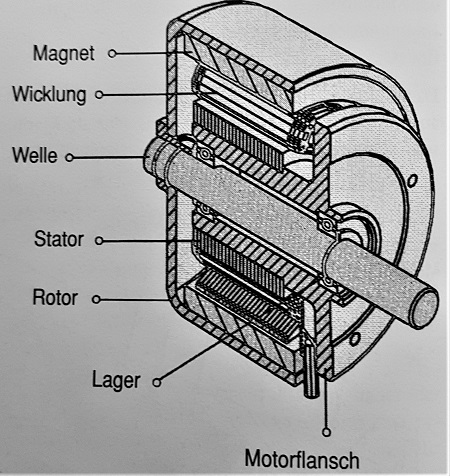
\includegraphics[width=6.5cm]{./Grafiken/3_2}
  \caption[Schnittbild eines BLDC-Motors in Außenläuferausführung]{Schnittbild eines BLDC-Motors in Außenläuferausführung (Quelle: \parencite[S.  76]{Stölting2011})}
  \label{fig:3_2}
\end{figure}

Der Stator besitzt im Gegensatz zum Innenläufer oft nur einen Flansch mit integriertem Legerohr. Somit entfällt das passgenaue Anfertigen sowie die fluchtende Montage zweier getrennter Flanschteile. Die beiden Kugellagersitze können in einer Aufspannung präzise gedreht werden. Für eine kostengünstige Fertigung der Wicklungen stehen Flyerwicklungsmaschinen mit äußerst kurzen Fertigungszeiten zur Verfügung. Bei konzentrierten Wicklungen besteht darüber hinaus die Möglichkeit der gleichzeitigen Wicklung verschiedener Stränge. Hohe Investitionen für Einzugs- und Wicklungsbandagierautomaten entfallen.

In Lüftern, Gebläsen und Ventilatoren wird die Motorelektronik üblicherweise auf einer Leiterplatte an der Flanschinnenseite des Motors integriert und durch den überlappenden Läufer geschützt.

Das Rotorgehäuse besteht bei Lüftern aus einem gezogenen, weichmagnetischen Blechkopf, der über eine Niet-, Schweiß- oder Spritzverbindung mit der Welle verbunden ist. Unter Einbezug des Topsbodens für die magnetische Flussführung lassen sich kleine Blechdicken und damit niedrige Gewichte realisieren. Die Magnete, bei lufttechnischen Applikationen meist kunststoffgebundene, elastische, anisotrope Ferritmagnetbänder oder bei Festplattenantrieben NdFeB-Magnetringe, werden in das Rotorgehäuse eingeklebt. Eine Bandage der Magente ist aufgrund des Rotormantels nicht erforderlich. Für extreme Fliehkraftanforderungen müssen zum Teil noch die Magnetseidenränder abgeschützt werden \parencite[S.  76--77]{Stölting2011}.

\subsection{Scheibenläuferausfürung}

Abbildung~\ref{fig:3_3} zeigt eine für Audio und Videogeräte bevorzugte Direktantriebsvariante in Einscheibenläuferausführung mit einer Leiterplatte als Spulen- und Elektronikträger, welcher in einem printmontierten ferromagnetischen Eisenrückschluss ausgeführt ist.

\begin{figure}[h]
  \centering
  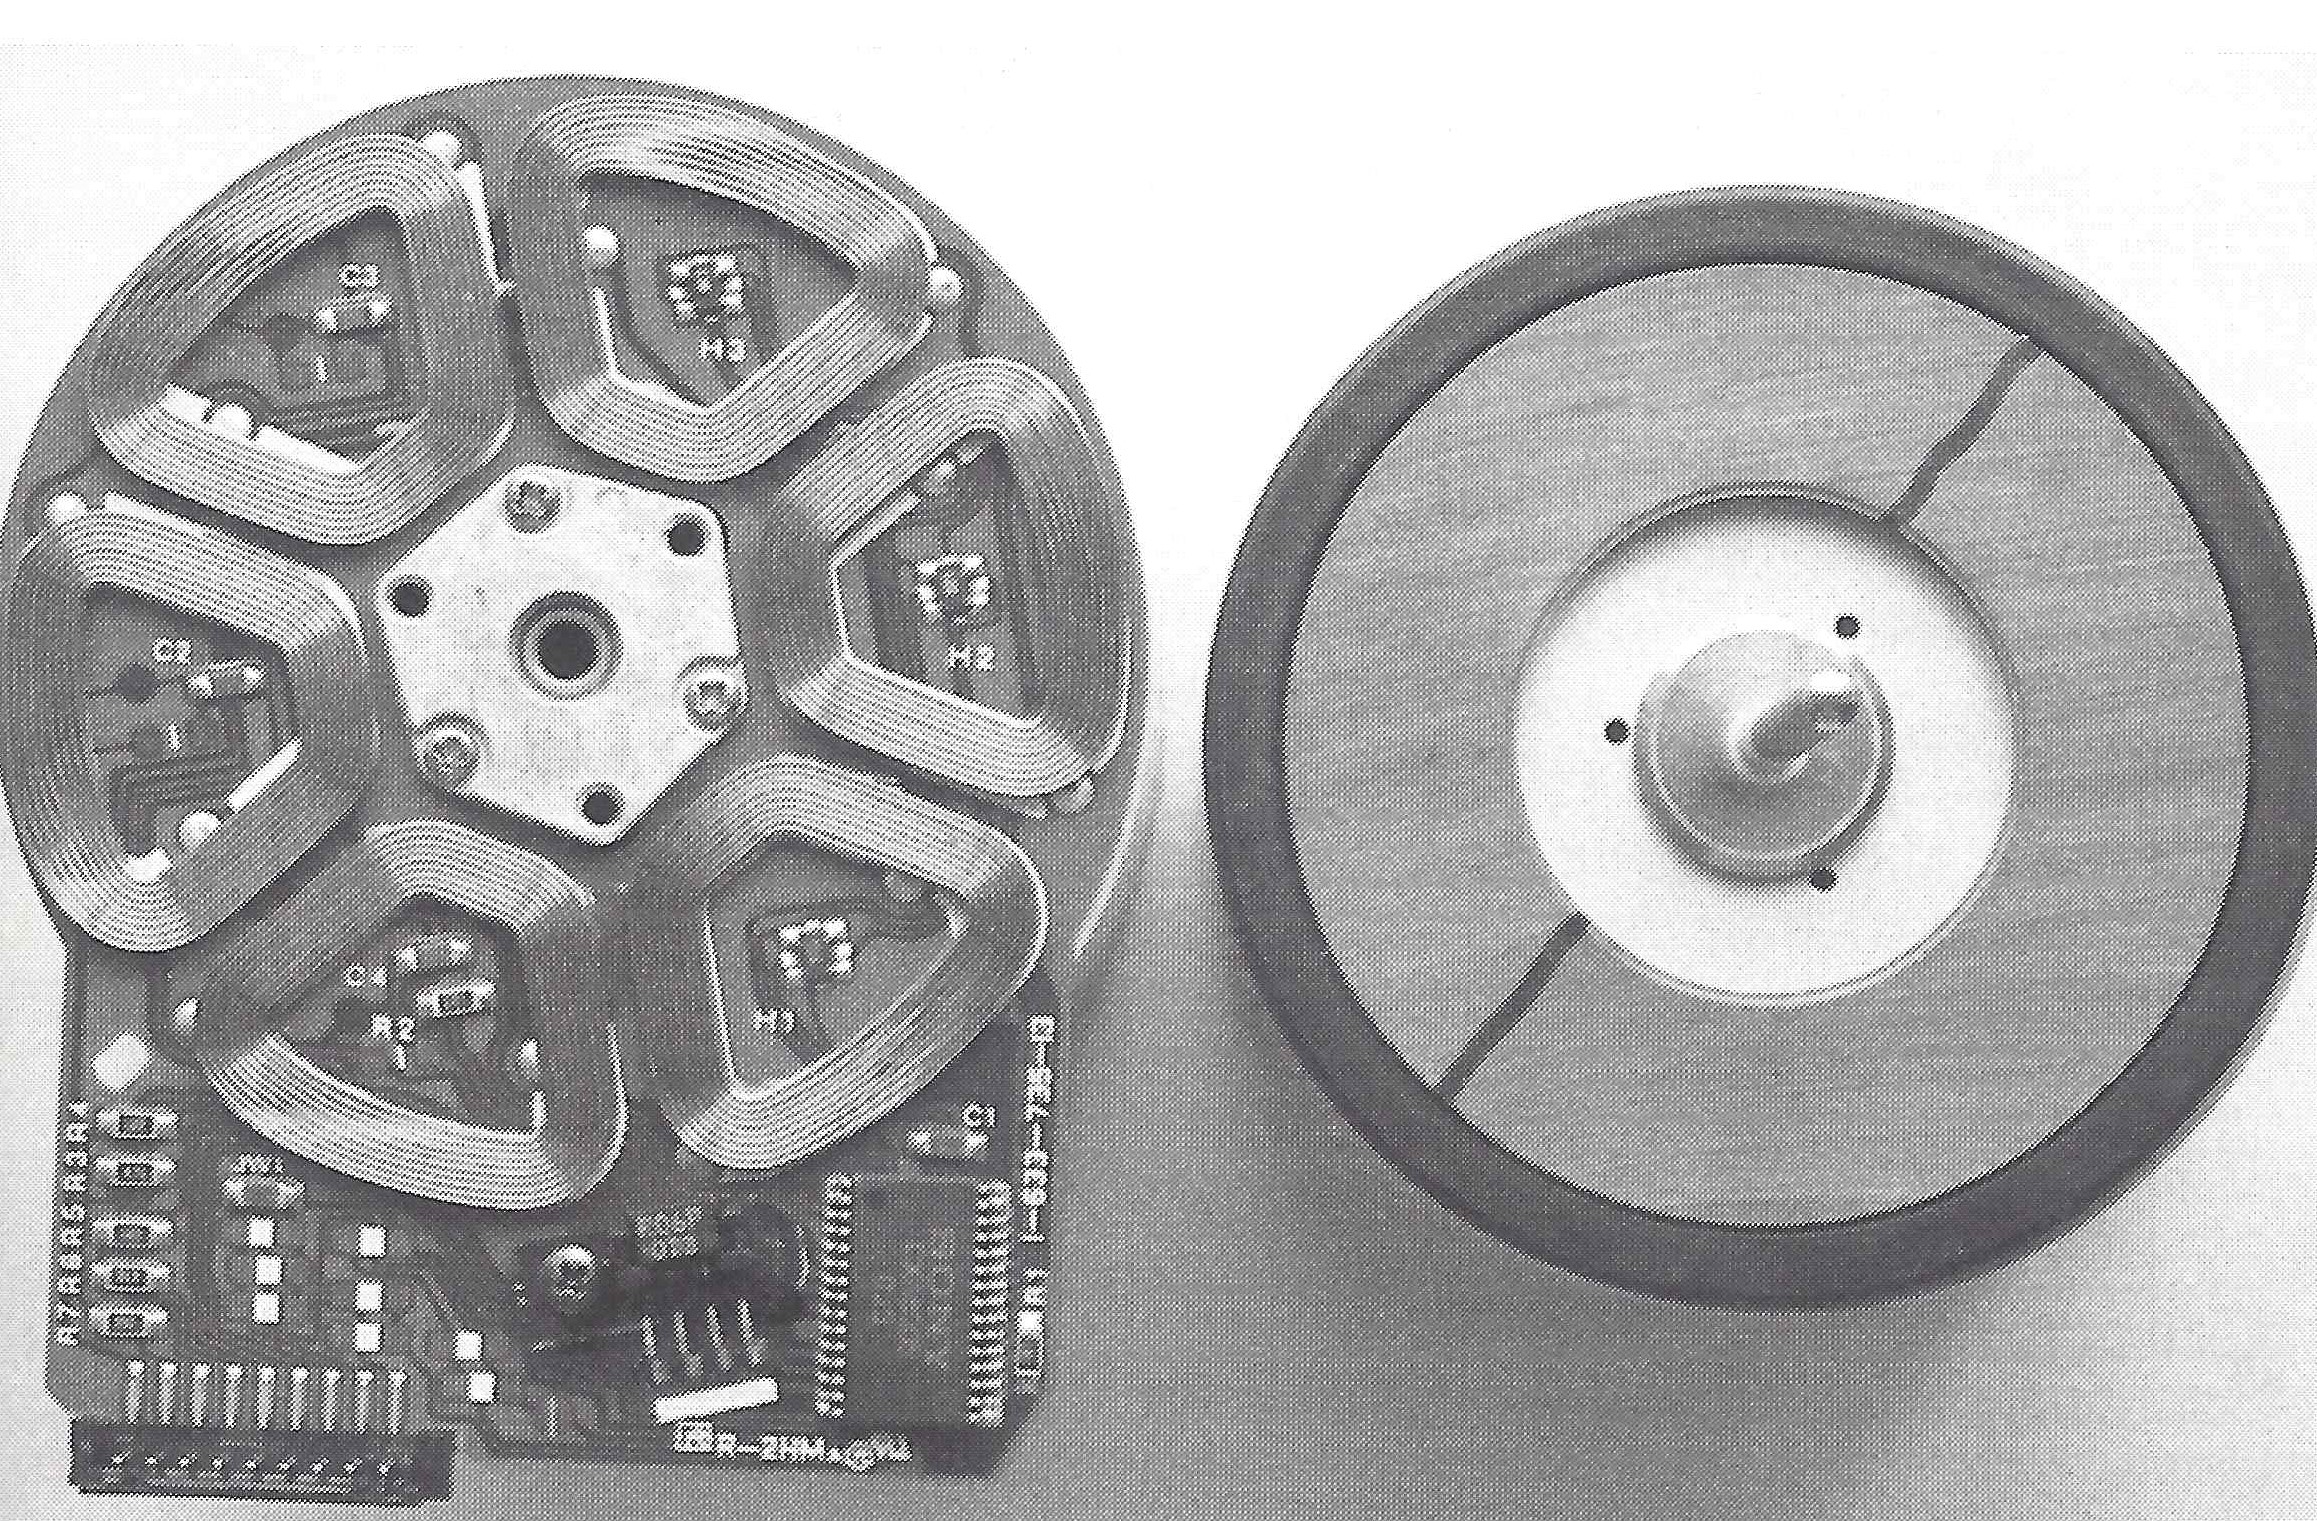
\includegraphics[width=9cm]{./Grafiken/3_3}
  \caption[BLDC-Motor in Scheibenläuferausfürung]{BLDC-Motor in Scheibenläuferausführung (Quelle: \parencite[S.  77]{Stölting2011})}%
  \label{fig:3_3}
\end{figure}

Für Anwendungen mit niedrigen Drehzahlen und Flussdichten genügt teilweise bereits ein einfaches Stahlblech als Statorjoch. Für höhere Ansprüche wird der ferromagnetische Rückschluss zur Begrenzung der Wirbelstromverluste mit einem kunststoffgebundenen Eisenpulververbundwerkstoff spiralförmig geblecht oder auch als mitrotierender (massiver) Rückschluss ausgebildet.

Mit dem bürstenlosen Scheibenläufer lassen sich in der dargestellten nutenlosen Ankerausführung in Verbindung mit einem hohen Rotorträgheitsmoment sehr gute Rundlaufwerte erzielen. Der Stator kann auch völlig eisenlos gefertigt werden, wenn die kunstoffumspritzte und damit selbsttragende Wicklung zwischen zwei über die Welle verbundenen Rotorscheiben angebracht ist. Die 2-Scheiben-Läuferausführung ist hierbei entweder symmetrisch mit zwei Permanentmagnetrotorscheiben oder asymmetrisch mit einer Permanetmagnetrotor- und einer Rückschlussscheibe ohne Magnete realisiert. Im Gegensatz zu der 1-Scheibenläuferbauweise treten hier keine technischen Problemstellungen hinsichtlich der dreidimensionalen Flussführung im Statoreisen sowie der hohen Lagerbelastung durch axiale Zugkräfte zwischen Stator und Rotor auf. Wicklungsseitig sind bei hohen Drehzahlen und hohen Polzahlen im Unterschied zu genuteten Wicklungsausführungen auch die durch das Permanentmagnetfeld erzeugte Wirbelstromverluste in den Spulendrähten (insbesondere bei großen Leiterquerschnitten) zu beachten.

Der Scheibenläufer eignet sich sehr gut für eine Integration von Motor und Motorelektronik und ermöglicht eine sehr kompakte Flachbauweise \parencite[S.  77--78]{Stölting2011}.

\subsection{Nutenloser BLDC-Motor}

Die bürstenlosen Premanentmagnetmotoren mit nutenloser, zylindrischer Wicklungsausführung sind den Glockenankerkommutatormotoren nachgebildet (S.  Abbildung~\ref{fig:3_4}). Die im Allgemeinen dreisträngige Rauten- oder Schrägwicklung ist im Luftspalt des Motors angebracht und wird in der Konstruktionsvariante von Abbildung~\ref{fig:3_4} innen von einem auf der Welle angebrachten Permanentmagneten und außen von einer ebenfalls auf der Welle montierten massiv ausgeführten Eisenjochglocke umschlossen. Durch die selbsttragende nutenlose Wicklung und den mitrotierenden Eisenrückschluss entstehen nahezu keine Eisenverluste im Motor. Dies wirkt sich insbesondere bei hohen Drehzahlen sehr günstig auf den Wirkungsgrad auS. 

\begin{figure}[h]
  \begin{minipage}{.48\linewidth}
    \centering
    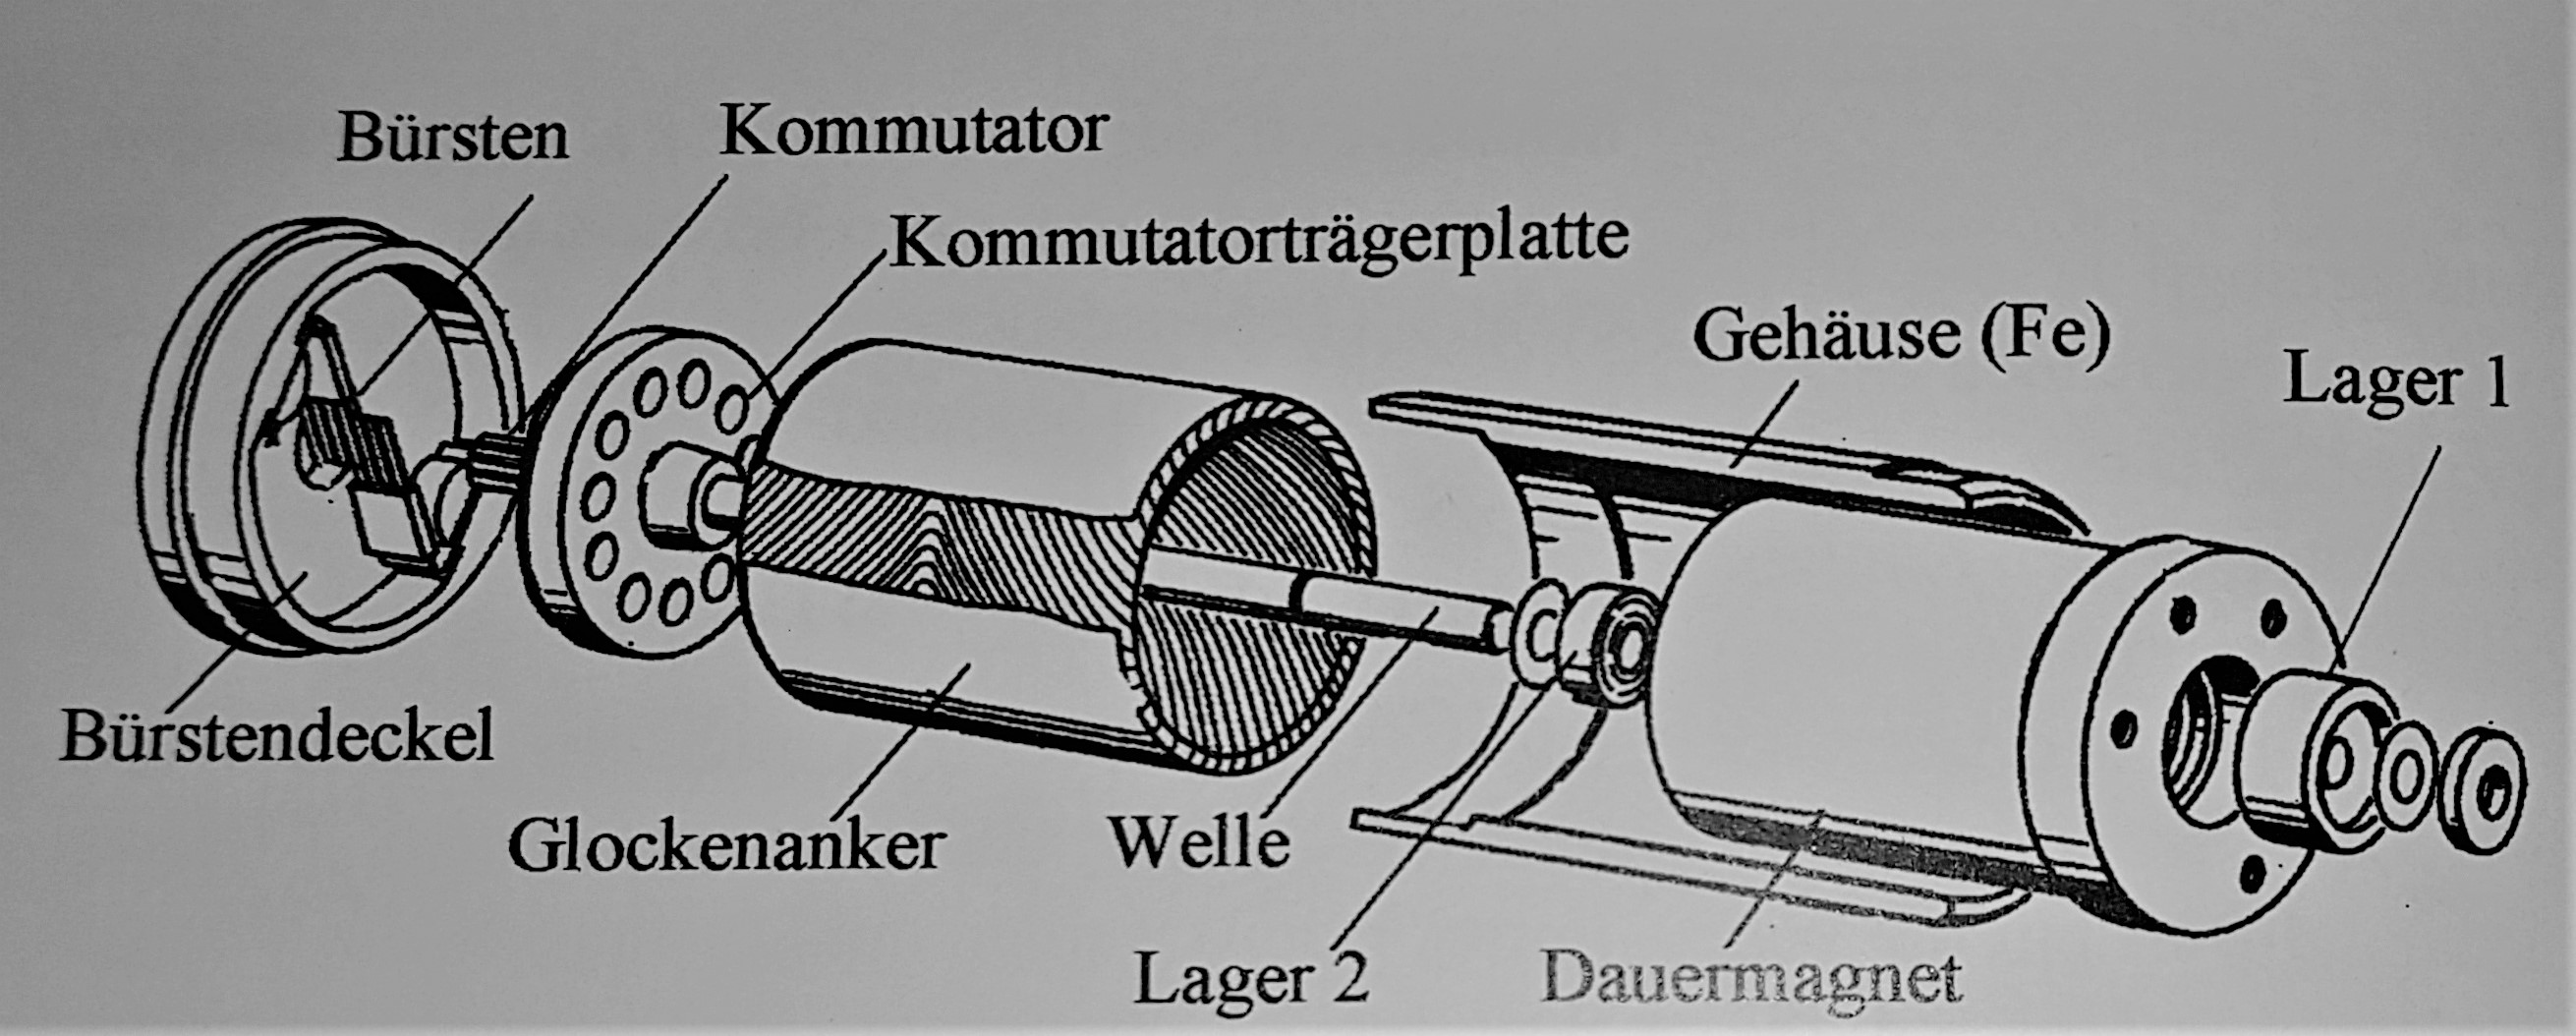
\includegraphics[width=\textwidth]{./Grafiken/3_4}
    \caption[Prinzipieller Aufbau des Glockenankerkommutatormotor]{Prinzipieller Aufbau des Glockenankerkommutatormotor (Quelle: \parencite[S.  30]{Stölting2011})}%
    \label{fig:3_4}
  \end{minipage}\hfill%
  \begin{minipage}{.48\linewidth}
    \centering
    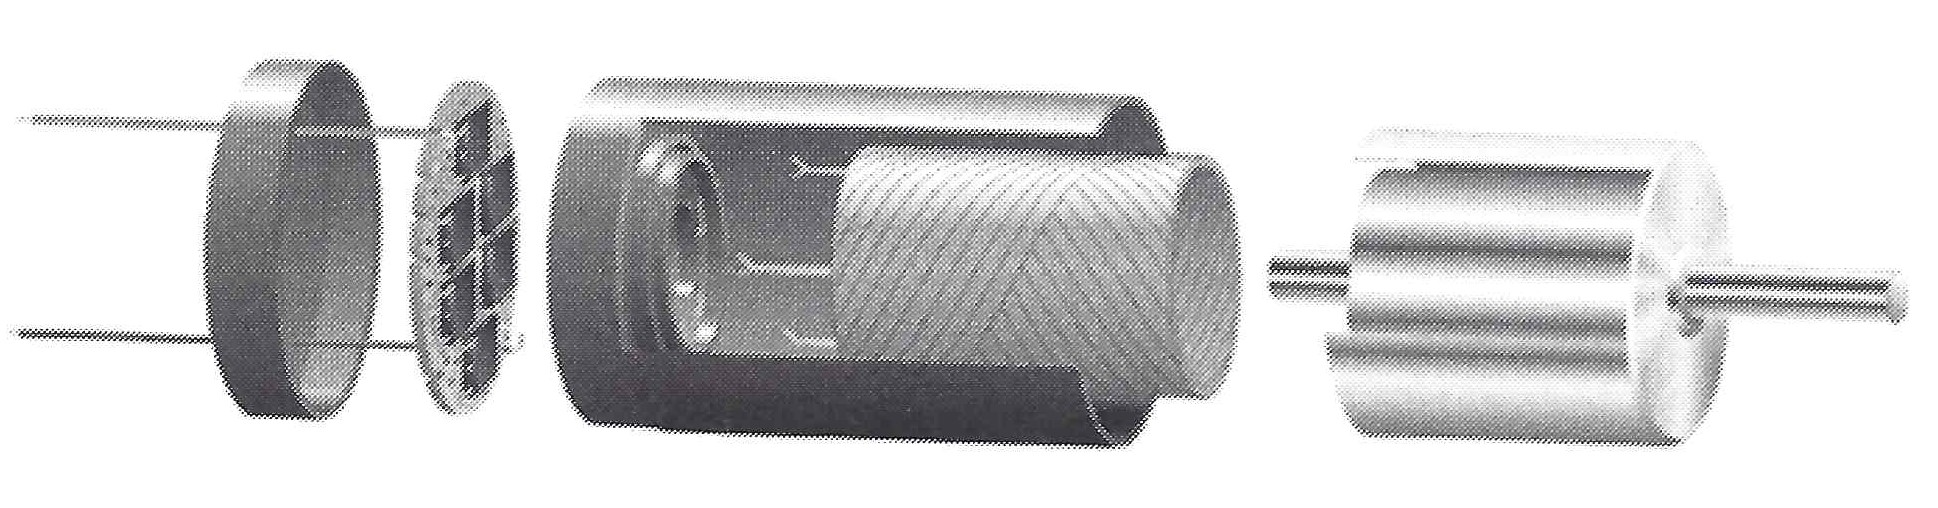
\includegraphics[width=\textwidth]{./Grafiken/3_5}
    \caption[Prinzipieller Aufbau des nutenlosen BLDC-Motors]{Prinzipieller Aufbau des nutenlosen BLDC-Motors (Quelle: \parencite[S.  78]{Stölting2011})}%
    \label{fig:3_5}
  \end{minipage}
\end{figure}

Die Lebensdauer der bürstenlosen Motoren mit freitragender Wicklung wird im Vergleich zu den Glockenankerkommutatormotoren lediglich durch die Lager und die Kommutierungselektronik bestimmt. Die Elektronik ist in einigen Ausführungen im Rückteil des Motorgehäuses integriert.

Sowohl die Wicklungsausführung als auch die diametrale Magnetisierung der zweipoligen Zylindermagnet führen zu sinusförmigen Flussverkettungen und damit zu sinusförmigen induzierten Polradspannungen. Dementsprechend ist hinsichtlich der Gleichförmigkeit des Drehmomentes eine sinusförmige Ansteuerung empfehlenswert. Im Gegensatz zu den Glockenankerkommutatormotoren, die aufgrund der hohen Spulenzahl trotz Blockkommutierung sehr geringe Drehmomentwelligkeitswerte erreichen, kann sich bei der nur dreisträngigen bürstenlosen Ausführung die Blockkommutierung für sehr anspruchsvolle Servo-Applikationen unter Umständen störend auswirken. Aus Kostengründen sowie aufgrund des beschränkten Einbauvolumens für Elektronik und Sensorik wird jedoch in vielen Anwendungen die Blockstromkommutierung der sinusförmigen Ansteuerung vorgezogen. Mit steigender Drehzahl verringern sich Unterschiede zwischen Sinus- und Blockkommutierung in den Drehzahlschwankungen aufgrund des glättenden Einflusses des Rotorträgheitsmomentes \parencite[S.  78]{Stölting2011}.

%%% Local Variables:
%%% mode: latex
%%% TeX-master: "BLDC"
%%% End:

\section{Typische Anwendungen des BLDC-Motors}

Viele Funktionen, die früher zum Aufgabengebiet der bürstenbehafteten Motoren gehörten werden mittlerweile von bürstenlosen Gleichstrommotoren erfüllt. Jedoch hindern Kosten und hoher Steuerungsaufwand den Motorentyp daran, seinen Vorgänger vollständig abzulösen.

Trotzdem dominieren BLDC-Motoren heutzutage besonders in Anwendungsgebieten, bei denen ein niederer Wartungsaufwand, hohe Motordrehzahlen, hohe Zuverlässigkeit und hohe Effizienz zu den Anforderungen gehören. Es folgt ein kurzer Überblick über die typischen Anwendungsgebiete des BLDC-Motors. Danach wird ein detailliertes Anwendungsbeispiel ausgeführt.

\subsection{Überblick}

\paragraph{Fortbewegungsmittel:} Mittlerweile finden sich bürstenlose Gleichstrommotoren in radgetriebenen Fahrzeugen jeglicher Größe. Vom elektrisch untertützten Fahrrad \parencite[S.6]{Xia2012} bis zum elektrisch angetriebenen Lastkraftwagen werden BLDC-Motoren in nahezu jedem Segment der Fortbewegungs- und Transportmittel eingesetzt. Eine mögliche Anwendung ist die Ausführung als Radnabenmotor, welche in Abbildung \ref{fig:Radnabenmotor} dargestellt ist.
\begin{figure}[h]
  \centering
  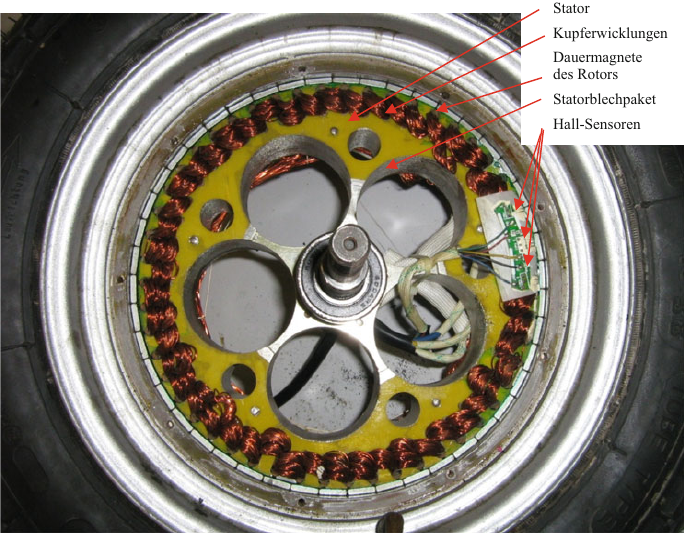
\includegraphics[width=10cm]{Radnabenmotor}
  \caption[Radnabenmotor]{Radnabenmotor (Quelle: \parencite[S.132]{Babiel2014})}
  \label{fig:Radnabenmotor}
\end{figure}
Hier kann besonders von der hohen Effizienz des Motors profitiert werden, da durch diese Eigenschaft höhere Batterielaufzeiten erzielt werden können \parencite[S.4]{Xia2012}. Da Elektromotoren hier nicht nur für den Antrieb des Fahrzeugs, sondern auch für Fensterheber, Airbags, Scheibenwischer, Schließmechanismen und vieles mehr genutzt werden können werden in einem durchschnittlichen Personenkraftwagen Dutzende, wenn nicht gar hunderte Elektromotoren verbaut \parencite[S.4]{Xia2012}.

\paragraph{Batteriebetriebenes Werkzeug:} Bei Anwendungen im handwerklichen Alltag werden bürstenlose Motoren besonders in Sägen, Bohrmaschinen, Laubgebläsen, Rasentrimmern und vielem mehr verwendet. Von vielen der genannten Maschinen finden sich auf der Baustelle kabelgebundene Versionen, die jedoch einige Nachteile mit sich bringen. Nennenswert wären zum Beispiel Kabelmanagement und die damit verbundene Not einer Stromversorgung, die bei einem Neubau oftmals erst durch einen kommunalen Stromverteiler gelegt werden muss. Durch die Verwendung von BLDC-Motoren verringert sich die Leistungsanforderung des Geräts drastisch, sodass nun Geräte mit Batterieversorgung entwickelt und gebaut werden können, die an einem zentralen Punkt der Baustelle nachgeladen werden können, ohne ein kompliziertes Netzwerk aus Stromverteilern und Verlängerungskabeln aufbauen zu müssen. Ein weiterer Vorteil liegt in der Gewichtsersparnis der Maschinen, denn durch die höhere Leistungsdichte eines BLDC-Motors kann ein kleinerer Motor bei selber Leistung verwendet werden. In der untenstehenden Abbildung \ref{fig:Vergleich} wird zudem der Größenunterschied gut sichtbar. Das bürstenlose Modell (rechts) kann weitaus kompakter gebaut werden und verfügt trotzdem über 50\% mehr Drehmoment (\SI{60}{\newton\meter})als das bürstenbehaftete Modell (\SI{40}{\newton\meter})

\begin{figure}[H]
  \centering
  %------------------------------
  \begin{minipage}{.49\textwidth}
    \centering
    \includegraphics[height=5cm]{Makita_Bürstenbehaftet}
  \end{minipage}\hfill%
  \begin{minipage}{.49\textwidth}
    \centering
    \includegraphics[height=5cm]{Makita_Bürstenlos}
  \end{minipage}
  \caption[Vergleich Akkubohrschrauber]{Vergleich zweier Akku-Bohrschrauber der Firma Makita. Links: Modell DDF451, bürstenbehafteter Antrieb, Gehäuselänge: \SI{238}{\milli\meter}. Rechts: Modell DDF481, bürstenloser Antrieb, Gehäuselänge: \SI{205}{\milli\meter}. (Quelle: Fa. Makita)}
  \label{fig:Vergleich}
\end{figure}

\paragraph{Haushaltsgeräte:} In der letzten Zeit wurden weltweit jährlich etwa 30\% mehr Elektromotoren in Haushaltsgeräten verbaut. Mit dem steigenden Lebensstandard der Menschen und dem wachsenden Umweltbewusstsein sind bürstenlose Gleichstrommotoren immer mehr das Mittel der Wahl im alltäglichen Gebrauch; so auch im Haushalt \parencite[S.6]{Xia2012}. Lüfter sind ein Anwendungsgebiet, in dem man mittlerweile ausschließlich bürstenlose Gleichstrommotoren vorfindet. Auch hier wird insbesondere von der Leistungsersparnis profitiert. Ein weiterer Vorteil im Segment der Lüfter und Ventilatoren (auch Haartrockner, Heizlüfter etc.) besteht in der Tatsache, dass die Lautstärke des Geräts abnimmt, da keine mechanische Reibung bei der Kommutation entsteht.

\paragraph{Modellfluggeräte:} Das Wachstum der Popularität von ferngesteuerten Modellfluggeräten --- insbesondere Drohnen und Quadrokoptern --- wurde maßgeblich durch die Entwicklung des BLDC-Motors angestoßen. Im Bereich der Fluggeräte wurden seither stets kleine Verbrennungsmotoren eingesetzt. In einigen Staaten wurden Verbrennungsmotoren für diese Anwendung mittlerweile verboten, da die Lärmverschmutzung als zu hoch eingestuft wurde. Auch hier zeigen sich die Vorteile des bürstenlosen Gleichstrommotors. Zusätzlich sorgt die Einsetzung dieses neuen Motortyps für eine höhere Reichweite, da eine kleineres Verhältnis von Gewicht und Leistung vorliegt.

\paragraph{Industrielle Anwendungen:} Im industriellen Umfeld spielt der BLDC-Motor insbesondere in der Produktion, sowie der industriellen Automatisierung eine große Rolle. Bürstenlose Motoren sind für diese Funktionen besonders gut geeignet, da sie sich durch eine hohe Leistungsdichte, hohe Effizienz, große Drehzahlbereiche und niederen Wartungsaufwand auszeichnen \parencite[S.8]{Xia2012}. In der Produktion werden sie vor allem für Bewegungsregelung, Positionierung und Aktorik verwendet.

\subparagraph{Bewegungsregelung:} Bürstenlose Gleichstrommotoren werden häufig als Treiber für Pumpen, Lüfter und Spindeln, beispielsweise in CNC-Fräsen eingesetzt. Aufgrund ihrer Konstruktion verfügen BLDC-Motoren über gute thermische Eigenschaften und eine hohe Effizienz. Hinzu kommt die niederere Massenträgheit im Vergleich mit dem bürstenbehafteten Motor. All dies sind Eigenschaften, die den BLDC-Motor für dieses Einsatzgebiet prädestinieren.

\subparagraph{Positionierungs- und Aktuatoriksysteme:} BLDC-Motoren werden als Aktorik- und Positionierungssysteme in der Industrie eingesetzt \parencite[S.159]{Gopal2002}. In diesem Anwendungsgebiet trifft man besonders bürstenlose Servo- oder Schrittmotoren an, beispielsweise in Industrierobotern. Darüber hinaus können bürstenlose Gleichstrommotoren auch dazu verwendet werden, Linearaktuatoren anzutreiben \parencite[S.91]{Zhang2013} (s. dazu auch Abbildung \ref{fig:Linearantrieb}).

\begin{figure}[h]
  \begin{minipage}{.49\textwidth}
    \centering
    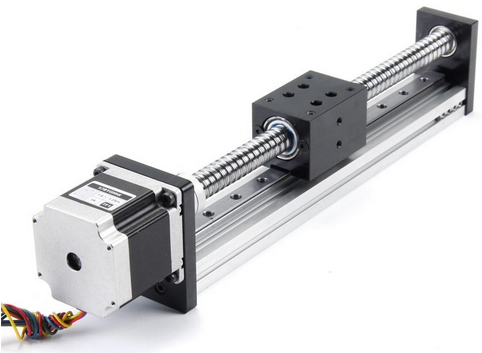
\includegraphics[width=\textwidth]{Linearantrieb}
    \caption[Linearantrieb mit BLDC-Motor]{Linearantrieb mit BLDC-Motor (Quelle: Fa. Banggood)}
    \label{fig:Linearantrieb}
  \end{minipage}\hfill%
  \begin{minipage}{.49\textwidth}
    \centering
    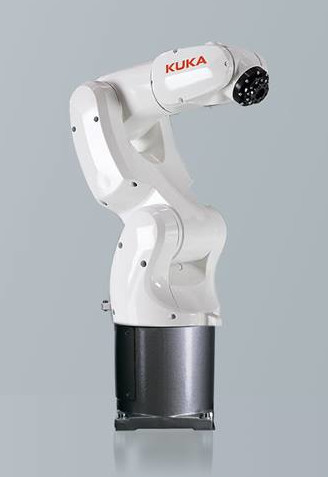
\includegraphics[height=7cm]{Industrieroboter}
    \caption[Industrieroboter KR 3 Agilus]{Industrieroboter KR 3 Agilus (Quelle: Fa. Kuka)}
    \label{fig:Industrieroboter}
  \end{minipage}
\end{figure}

Im nächsten Abschnitt wird der Einsatz von bürstenlosen Gleichstrommotoren exemplarisch am Beispiel eines Industrierobotersystems vorgestellt.

\subsection{Ausführliches Anwendungsbeispiel}

%%% Local Variables:
%%% mode: latex
%%% TeX-master: "BLDC"
%%% End:

% \chapter{Ausführliches Anwendungsbeispiel}

%%% Local Variables:
%%% mode: latex
%%% TeX-master: "BLDC"
%%% End:

\section{Fazit}

Bürstenlose Gleichstrommotoren nehmen einen sehr vielfältigen und vielversprechenden Bereich in heutigen Aktorikanwendungen ein. Man findet Sie in verschiedensten Ausführungen, Größen und Anwendungsgebieten in nach wie vor ansteigenden Stückzahlen vor. Dieser Zustand wird sich 

%%% Local Variables:
%%% mode: latex
%%% TeX-master: "BLDC"
%%% End:


\clearpage
\printbibliography[title=Literaturverzeichnis]%

\end{document}

%%% Local Variables:
%%% mode: latex
%%% TeX-master: t
%%% End:
